An important consideration for migration and consolidation related
decisions is the VM's resource requirement on the target host. 
%For mutually communicating VMs, 
%consolidation into a colocated set and migration to dispersed
%placements, can result in different CPU requirements.
VMs that mutually communicate are said to have \textit{network affinity}
and when VMs migrate, they may get colocated or dispersed w.r.t each 
other\textemdash{}resulting in different CPU overheads for network communication.
Network traffic between colocated VMs is considered \textit{intra-PM}, 
whereas between dispersed VMs is \textit{inter-PM}. Given a 
communicating VM pair, migration of one may cause change of network traffic
between them from \textit{inter-PM} to \textit{intra-PM},
or vice versa, depending on whether they get colocated or dispersed,
respectively\textemdash{}this is referred to as the \textit{mutable} nature 
of network affinity.
%due to \textit{mutable} nature of \textit{network affinity} between them.
In this work, we build
\emph{affinity-aware} models to predict expected CPU
requirements upon colocation or dispersion of VMs.
We make the following
contributions,
\begin{itemize}
		\singlespacing
%\vspace{-0.05in}
\vspace{-0.1in}
\item \emph{Event profiling} of intra-PM and inter-PM network 
	communication paths in Xen. % using \texttt{Xenoprof}~\cite{xenoprof}.
\item \emph{Benchmarking} of CPU usage
of VMs (Xen and KVM) for various workloads
in colocated and dispersed configurations.
\item Development of \emph{affinity-aware pair-wise} models to predict \textit{total}
	as well as \textit{differential} CPU usage, when a pair of VMs move between
	dispersed and colocated configurations.
%\item Apply above pair-wise models to \emph{multi-VM scenarios}, where
%a single migrating VM has more than one neighboring
%VMs with which it exhibits network-affinity, both on source \& target PMs.
\item Apply the pair-wise models to \textit{multi-VM scenarios} to predict CPU usage of a set of VMs.
\item \emph{Comprehensive evaluation} using synthetic workloads \& 
	benchmark applications, for pair-wise models as well as multi-VM scenarios.
\end{itemize}

%\subsection{Profiling study of Xen I/O virtualization}
%Using the tool \texttt{Xenoprof}~\cite{xenoprof}, we performed
%event monitoring for network transmission between a pair of Xen-based
%VMs in both colocated and dispersed scenarios.
%%~\cite{xen-internals, xen-networking, linux-networking}.
%%A common optimization in the colocated case is that packet 
%%check-summing is discarded, under the assumption that
%%memory copying (performed in colocated case) is quite reliable relative
%%to physical network transmission (corresponding to dispersed case).
%Colocated Xen-based VMs are
%connected to a layer 2 software bridge, so local network
%transmission is achieved via shared memory.
%However, network transmission between dispersed
%VMs is additionally
%DMA-copied\nomenclature{DMA:}{Direct Memory Access}\index{DMA}
%into the network interface
%card's (NIC\nomenclature{NIC:}{Network Interface Card}\index{NIC})
%buffer, and transmitted.
%Upon reception, packet is copied
%from NIC buffer into kernel buffer 
%and interrupt sent to host's driver domain (Dom0).
%The packet is subsequently inspected by Dom0
%and destination VM is notified. 
%Thus, end-to-end communication path is significantly longer in 
%dispersed case than colocated case.
%%These differences in CPU overheads were also observed empirically with
%both Xen and KVM environments, as presented next.

\subsection{Micro-benchmarking the effect of colocation on CPU Usage}
It is discussed in~\cite{virtual-putty}
that colocated provisioning can result in changes in
resource usage\textemdash{}however, empirical quantification is lacking.
We address the following questions,
(i) For communication between dispersed VMs, what is the 
change in CPU usage when VMs get colocated? 
(ii) For other network traffic and workloads, is colocated CPU usage a 
summation of dispersed usages?
%(iii) For pure CPU or disk workloads, is colocated CPU usage
%a summation of dispersed usages? 

%\begin{figure}[t]
%	\centering
%	\subfloat[Xen setup]{\includegraphics[scale=0.575]{jss-figures/benchmark}}
%	~~~~~~~~~~~~~~~~~~~~
%	\subfloat[KVM setup]{\includegraphics[scale=0.575]{jss-figures/kvmbenchmark}}
%	\caption{Setup for benchmarking, profiling and model evaluation.}
%	\label{fig:setup}
%\end{figure}

\begin{figure}
	\RawFloats
	\begin{minipage}{0.45\textwidth}
		\centering
		\includegraphics[scale=0.575]{jss-figures/benchmark}
		\caption{Setup for benchmarking, profiling and model evaluation.}
		\label{fig:setup}
	\end{minipage}
	\begin{minipage}{0.5\textwidth}
		\centering
		\includegraphics[scale=0.9]{arescue-figures/aff-benchmark/domU-cpu-vs-affine-rx-curve.eps}
		\includegraphics[scale=0.9]{arescue-figures/aff-benchmark/dom0-cpu-vs-affine-curve.eps}
		\caption{CPU utilization due to \textit{mutable} network traffic (in Xen setup).}
		\label{fig:cpuovhd-rxtx}
	\end{minipage}
\end{figure}	

%\vspace{-0.2in}
%\paragraph{Custom Micro-benchmarks:}
%We developed a multi-threaded load generation 
%tool, \texttt{LoadGen}, that generates
%CPU-intensive, network-intensive, disk-intensive and mixed workloads.
%Workloads are generated using a client-server setup,
%wherein a \textit{client} (the controller machine) remotely connects to
%the \textit{servers} (VMs), and invokes \texttt{LoadGen} command
%to generate desired workload.
%\vspace{-0.2in}
\paragraph{Setup:}
We developed a multi-threaded load generation 
tool, \texttt{LoadGen}, that generates
CPU-intensive, network-intensive, disk-intensive and mixed workloads.
We performed benchmarking for both Xen and KVM.
Fig.~\ref{fig:setup} shows the experimental setup that we
%The setup used for benchmarking with Xen virtualization technology
%is as shown in Fig.\ref{fig:setup}(a) wherein Dom0 is the privileged
%domain as described earlier in 
%Section~\ref{sec:litreviewchap-io-virtualization}.
%In case of KVM platform,
%there is no management domain since it
%does not follow the driver domain I/O model. Hence, the setup
%for KVM benchmarking is a slightly modified version, as
%depicted in Fig.~\ref{fig:setup}(b).
%As shown in the setup of Fig.~\ref{fig:setup}, 
used\textemdash{}two PMs host the VMs, and
each PM is connected via a Layer-2 Switch to an NFS server which hosts
the VMs' virtual disk images.
%disk images associated with the VMs. 
%Thus, all disk read/write
%operations are NFS-read/write operations which generate network traffic
%at the host. 
The Layer-2 Switch and all network links of the
machines operate at 100 Mbps.
The Controller uses scripts to automate
load generation and resource-usage measurements.
%Load generation is done using an automated script residing at the Controller,
%that invokes a custom application program (called \texttt{LoadGen})
%at each VM.
%Resource usages are measured using utilities like 
%\texttt{Xentop} (for Xen), %~\cite{xentop} (for Xen),
%\texttt{top} (for KVM),
%\texttt{sar}, and %~\cite{sar}, 
%\texttt{iptables}. %~\cite{iptables}.

%\begin{figure}%
%	\hspace{-0.3in}
%	\subfloat[DomU CPU utilization for Rx]{\includegraphics[scale=0.9]{arescue-figures/aff-benchmark/domU-cpu-vs-affine-rx-curve.eps}}
%%	\subfloat[DomU CPU utilization for Tx]{\includegraphics[scale=0.9]{arescue-figures/aff-benchmark/domU-cpu-vs-affine-tx-curve.eps}} \\
%	\centering
%	\subfloat[Dom0 CPU utilization for Rx/Tx]{\includegraphics[scale=0.9]{arescue-figures/aff-benchmark/dom0-cpu-vs-affine-curve.eps}}%
%	\caption{CPU utilization due to \textit{mutable} network traffic (in Xen setup).}
%	\label{fig:cpuovhd-rxtx}
%\end{figure}
%

\vspace{-0.4in}
\paragraph{Benchmarking results:}
%Hence we perform this benchmarking study of effect of
%network-affinity between two VMs\textemdash{}VM1
%and VM2 act as a Tx/Rx pair to transmit and receive data
%at different rates. 
%To study the implications of network-affinity
%between VMs, the experiment is conducted in both
%colocated and dispersed scenarios. The CPU utilization levels of both
%Dom0 and DomU are measured (refer Fig.~\ref{fig:cpuovhd-rxtx}).
Fig.~\ref{fig:cpuovhd-rxtx} plots DomU and Dom0 CPU utilization 
for varying network usage between a pair of VMs (i.e., \textit{mutable} 
traffic), in colocated
and dispersed scenarios. %\textemdash{}VM1 and VM2 form a Tx/Rx pair.
%As can be seen, with increase in network usage, benefits of VM colocation
%increase. 
At 90 Mbps, the colocated DomU utilization is 10\%,
which is almost half of the dispersed case.
%For the transmitting VM, the CPU utilization shows
%a decrease but very marginal.
%With close to 90 Mbps bandwidth utilization, the colocated
%CPU utilization is 10\%.
% This implies that there is definitely
% no increase in CPU utilization due to colocation of two 
% communicating VMs.
%Further, the absolute usage by Rx-network traffic is more
%than Tx-traffic for the same bandwidth\textemdash{}CPU utilization
%of 17\% and 9\% respectively, at 90 Mbps network bandwidth
%utilization.
%Fig.~\ref{fig:cpuovhd-rxtx}(b) shows corresponding Dom0 CPU usage.
Further, at 40 Mbps and 90 Mbps,
the difference in Dom0 CPU usage between
dispersed and colocated scenarios is 14\% and 25\%, respectively.
%dispersed (summation of utilization levels at both PMs in the
%dispersed scenario) and colocated (single
%Dom0 CPU) scenarios is 14\% and 25\%, respectively.

From our benchmarking, we concluded that differences in CPU usage across
colocated and dispersed placements occurs only for 
VMs that are mutually communicating, i.e., \textit{mutable} traffic. 
For workloads like CPU/disk workloads and 
\textit{immutable} traffic, different placements do not
affect CPU usage. 
Further, resource utilization and Dom0/DomU CPU utilization are linearly
related.

\subsection{Linear regression modeling for CPU requirement estimation}
%We run a set of benchmarks, also referred to as micro-benchmarks, in both
%scenarios\textemdash{}dispersed and colocated\textemdash{}which exercise the utilization
%levels of VMs along different
%axes\textemdash{}CPU, intra-PM and inter-PM network traffic, disk read and
%write operations.
\underline{Colocation and Dispersion models}:
We develop pair-wise CPU estimation models
that can predict total CPU requirement in target scenario
based on source scenario's resource usages. 
Specifically, using resource usage measurements of dispersed 
case, the ``colocation'' model predicts CPU utilization for 
colocated scenario, and based on resource usage in colocated case,
the ``dispersion'' model predicts for dispersed scenario.

Our benchmarking revealed that only the mutable network usage
causes changes in CPU requirement, upon a VM migration.
Hence, we build models to use \underline{two approaches of prediction}:-
(i)~Predict \textit{total} CPU requirement based on multiple 
resource usage profiles\textemdash{}CPU, disk and network,
(ii)~Predict \textit{differential} CPU requirement based only on
mutable network traffic metrics\textemdash{}later, take summation
of prediction with the source scenario's CPU usage to estimate
the total CPU requirement. Next, we briefly explain both the
approaches.

\subsection*{Approach 1: Prediction of total CPU requirement}

\paragraph{Intuition:} 
The total CPU requirement of a virtual machine accounts for all its 
activities, including usage of all other resources. Hence, this model
has all resource metrics as its
parameters: (i) $4$ metrics for mutable and
immutable transmit and receive network rates,
(ii) $3$ CPU metrics of \texttt{iowait}, \texttt{system}
and \texttt{user} CPU, and
(iii) $4$ metrics for disk read/write rates.
%blocks/second and bytes/second. 
%Since the correlation of all resource usages to CPU usage is linear, we employ
%linear regression methods to build the CPU estimation models.

\vspace{-0.2in}
\paragraph{Method:} We use multi-linear regression modeling, wherein
%Using values from the collected profiling data,
%the colocated CPU usage is represented as
%a linear function of the individually profiled resource metrics
%in the corresponding dispersed scenario (i.e. dispersed scenario
%stressed with the same workload),
%and similarly dispersed CPU usage is represented as a linear function of
%the colocated resource usage metrics.
the relation between estimated CPU and resource parameters is captured, 
as shown in Eqn. (\ref{mlr-eqn-1}).
\vspace{-0.2in}
\begin{equation}
\mbox{CPU}^{i}_{estimated} = C_{0} + C_{1} \times M^{i}_{1} + C_{2} \times M^{i}_{2} + ... + M^{i}_{m}
\label{mlr-eqn-1}
\end{equation}

\vspace{-0.2in}
\noindent where, $i$ is an iterator over each sample point,
$m$ is the number of parameters, $M^{i}_{j}$ is
the value of parameter $M_{j}$ collected in the sample point number 
$i$, and $\mbox{CPU}^{i}_{estimated}$ is the CPU usage
either after dispersion or after colocation of VMs.
%Thus, there are $11$ metrics in all to be considered.
% in Table~\ref{metrics-table}. 
%We build models for both DomU and Dom0 using the above multi-linear regression approach.
%Both the colocation and dispersion models for DomU have these $11$ parameters.
%The Dom0 \textit{colocation} model is built with metrics of both 
%DomUs\textemdash{}has $22$ parameters.
%The Dom0 \textit{dispersion} model
%depends on only one DomU's metrics at a time, and hence has only $11$
%parameters.
%For model building, we used 956 sample points in total\textemdash{}200 points 
%for CPU workload, 96 points for mutable network, 182 points
%for immutable network, 162 points for disk read, 158 points for disk write 
%and 158 mixed workloads.
To solve for the $m+1$ coefficients $C_{k}$, we use
Robustbase package, part of the R statistical computing environment.
%, for robust linear regression.
%The linear regression solver, takes as input $M^{i}_{j}$ values for the
%various workloads and outputs values of $C_{k}$ of best predict CPU utilization.
%The set of coefficients thus
%derived is the model that describes the relation between the $k$ parameters
%and the DomU and Dom0 colocated/dispersed CPU usage.

\subsection*{Approach 2: Prediction of differential CPU requirement}

\paragraph{Intuition:} The difference in CPU usage upon transition between
colocated and dispersed placements of a VM pair, depends only on the mutable
network affinity between them. Hence, we can predict only
the difference, and sum it with the original scenario's CPU usage, to
obtain the total CPU requirement.
The model parameters are bit-rates (in Kbps) and 
packet-rates (in packets per second) for both 
transmission (Tx) and reception (Rx), thus four parameters
in all. %: (i) Rx Kbps, (ii) Rx pkts/s, (iii) Tx Kbps, and (iv) Tx pkts/s. 
%Note that differential Dom0
%CPU is the difference in CPU usage between that incurred for the single (colocated) Dom0 and
%the summation of both (dispersed) Dom0.

\vspace{-0.2in}
\paragraph{Method:} 
Formally, Eqn. (\ref{cpu-diff-eqn}) captures the
general notion of change in CPU usage %($\Delta\mbox{CPU}$)
while transitioning between colocated and dispersed scenarios.
\vspace{-0.2in}
\begin{equation}
	% \hspace{-0.3in}
	\Delta\mbox{CPU} = \mbox{CPU}^{scenario1} - \mbox{CPU}^{scenario2}
	\label{cpu-diff-eqn}
\vspace{-0.2in}
\end{equation}
where, scenario$\{1|2\}$ = $\{colocated|dispersed\}$.
Each DomU and Dom0 model represented as
\vspace{-0.2in}
\begin{equation}
	\hspace{-0.3in} \Delta\mbox{CPU}_{est} = C_{0} + C_{1} \mbox{MutRx}_{Kbps} + C_{2} \mbox{MutRx}_{p/s} \\ 
	+ C_{3} \mbox{MutTx}_{Kbps}  + C_{4} \mbox{MutTx}_{p/s}
	\label{mlr-eqn}
\vspace{-0.2in}
\end{equation}
where, ``MutRx'' and ``MutTx'' stand for mutable network receive and transmit 
traffic, respectively. Once again, the Robustbase package %~\cite{robustbase}
is used to solve for the model coefficients.


\begin{figure}
\begin{floatrow}
\ffigbox{%
	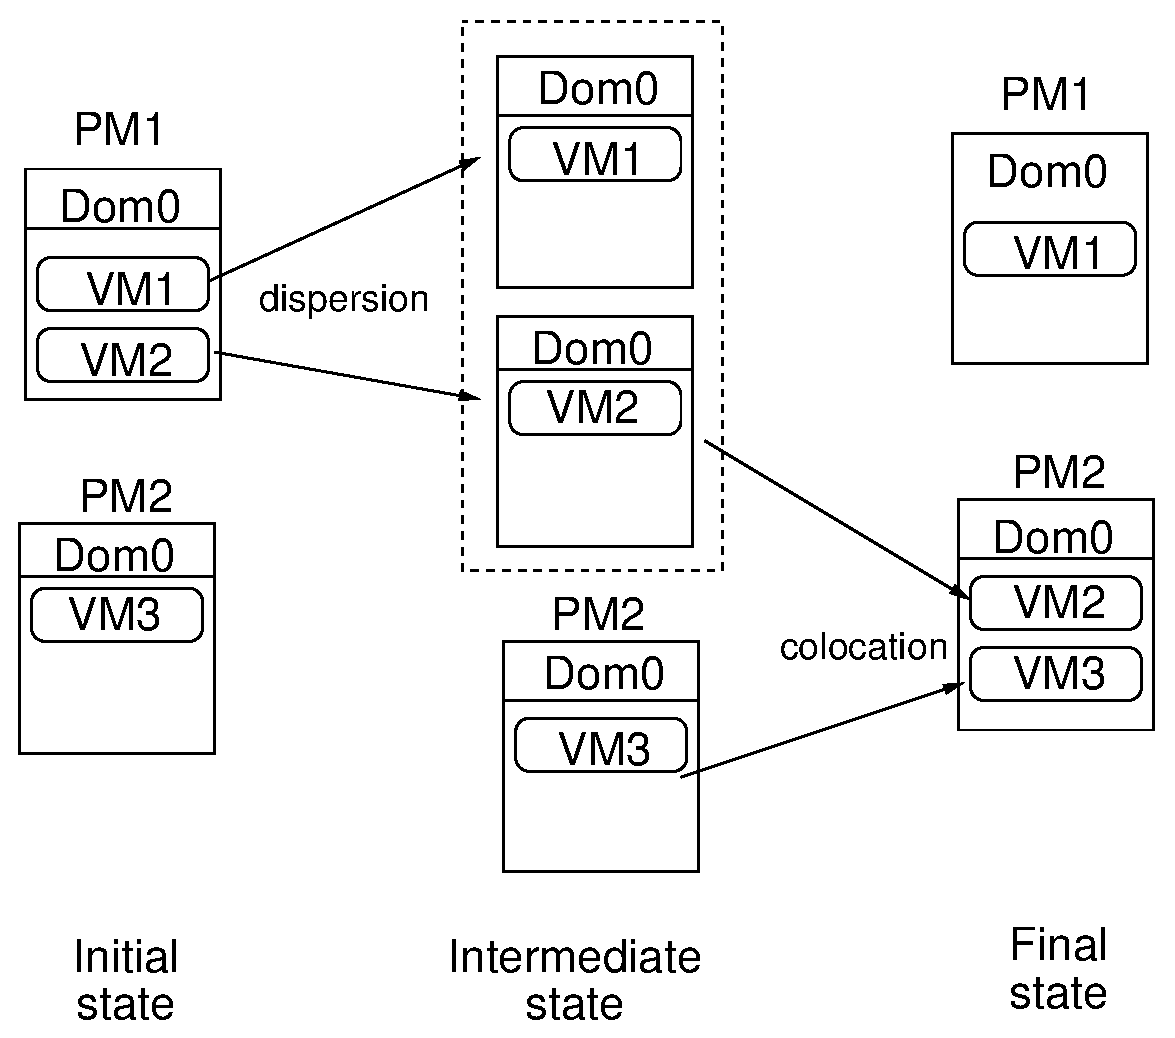
\includegraphics[scale=0.4]{jss-figures/new-forward-plus-rev.eps}
}{%
	\caption{Combined transition for $VM2$}
	\label{fig:forward-plus-reverse}
}
~~~
\vspace{-0.1in}
\small
\capbtabbox{%
	\begin{tabular}{|c|c|c|c|c|} \hline
		\textbf{Num} & \textbf{Max}  & \multicolumn{3}{|c|}{\textbf{Max error(\%CPU)}} \\  \cline{3-5}
	\textbf{of } & \textbf{n/w} & \textbf{DomU} &  \textbf{Dom0} & \textbf{Dom0} \\
    \textbf{clients} & \textbf{traffic} &  &  \textbf{colo} & \textbf{disp} \\ 
	\textbf{} & \textbf{(Mbps)} & \textbf{} &  \textbf{} & \textbf{} \\ \hline  %\cline{2-9}
  500 & 6.8 & 1.73 & 1.33 & 0.90 \\
	1000 & 13.4 & 1.50 & 0.98 & 0.82 \\
	1500 & 19.8 & 1.42 & 0.69 & 0.90 \\
	2000 & 26.4 & 0.90 & 1.08  & 1.21 \\
	2500 & 32.6 & 1.03 & 1.29 & 1.27 \\
	3000 & 39.4 & 1.36 & 1.50 & 1.54 \\ \hline
	\end{tabular}
}{%
	\caption{Model accuracy with varying load}
	\label{tab:xennumclients}
}
\end{floatrow}
\end{figure}

\subsection{Applying the pair-wise models to multi-VM scenarios}
%In a multi-VM scenario, any VM (say $VM_{x}$)
%may have multiple communicating neighbors, each belonging to
%exactly one of three sets, (i) \textit{affinity-at-source}
%(ii) \textit{affinity-at-target}, and (iii) \textit{affinity-at-other}.
%Migration of $VM_{x}$ will cause it to become dispersed from
%its \textit{affinity-at-source} set and colocated with its
%\textit{affinity-at-target} set\textemdash{}causing change in their CPU utilization.
In an example multi-VM scenario as shown in Fig.~\ref{fig:forward-plus-reverse},
migration of $VM2$ can cause it to be dispersed from $VM1$
and become colocated with $VM3$---we refer to this 
as a ``combined'' transition.
%Our aim is to predict the resource usage of all affected VMs and PMs.
%In Fig.~\ref{fig:forward-plus-reverse},
%CPU usages for $VM1$, $VM3$ and $PM1$ can be predicted by
%straight-forward application of \textit{colocation} and
%\textit{dispersion} models.
Here, CPU requirement estimation for $VM2$ and $PM2$ needs a
\underline{multi-phase prediction} methodology.
We need to first apply the \textit{dispersion model} to the
measured metrics corresponding to network-affinity level between $VM2$
and $VM1$, to get an intermediate estimate, and then apply the
\textit{colocation model} to the intermediate estimate
%This is an intermediate estimate and is used 
based upon network-affinity level
between $VM2$ and $VM3$ to get the final estimate.
%Intuitively,
%VMs in the \textit{affinity-at-other} set do not affect CPU
%requirement of the migrating $VM2$ because the nature of network-affinity
%between them stays the same (\textit{immutable}) both before and
%after migration.

\vspace{-0.1in}
\subsection{Summary of Experimental evaluation}
We generated CPU, disk, network and combinational workloads of
randomly picked levels to form our testing dataset.
Further, we used an application benchmark (RUBiS) to
perform testing\textemdash{}we generated different
levels of network traffic by using different number
of clients in each workload. Finally, we conducted
experiments with multi-VM scenarios wherein every
VM migration results in a different placement configuration,
and used the multi-phase prediction methodology 
to predict for every VM and PM.
Here, we present a list of main results. %subset of our results.

\begin{enumerate}
\singlespacing
	\item For both the approaches 1 and 2, we performed evaluation
with synthetic datasets and observed that Approach 1 (prediction 
of total CPU) had higher error of 4-5\% as compared to 
Approach 2 (prediction of differential CPU) error of 2\%.
	\item We conducted experiments with various number of clients
in RUBiS~\cite{rubis} and found maximum error
in each case to be within 2\% absolute CPU (refer Table~\ref{tab:xennumclients}). 
%This is tabulated in Table~\ref{tab:xennumclients}\textemdash{}maximum
%error is within 2\% absolute CPU.
	\item We created a 3-tier RUBiS setup and used the multi-phased
prediction methodology to predict the CPU usage of VMs and PMs 
across multiple transitions, and found maximum estimation error
within 2\% absolute CPU.
\end{enumerate}

%For further evaluation of our prediction models, we
%chose RUBiS~\cite{rubis}. It is 
%a two-tier application, consisting of a web tier and a database tier
%that communicate with each other for servicing user requests. Each tier
%is hosted in a separate VM.
%We generate repeatable RUBiS workloads in both dispersed and colocated cases,
%and compare average resource usages (predicted versus measured)
%over 30-second intervals. 
%The workload consisted of 800 clients
%generating site browsing load simultaneously, and requests being fired
%at determined times.
%We present a subset of our results here.

%\begin{figure}[h]
%	\centering
%	\includegraphics[scale=0.525]{jss-figures/rubis-3tier-layout.eps}
%	\caption{RUBiS 3-tier setup with proxy, webserver and database}
%	\label{fig:threetier}
%\end{figure}
%
%\vspace{-0.2in}
%\paragraph{Estimating CPU usage for ``combined'' transitions:}
%Fig.~\ref{fig:threetier} depicts our
%three-tier setup\textemdash{}we use Muffin proxy as the first tier of our test application.
%We consider a series of VM migration steps, each resulting in a different
%VM placement during a RUBiS run with 1000 clients.
%%and we apply \emph{colocation} and \emph{dispersion} models
%%appropriately to derive CPU usage prediction for each VM and PM. The series
%%of VM migration steps are 
%%(refer Fig.\ref{fig:migration-steps}):
%(a)~\textit{C0}: all 3 VMs on different PMs each (i.e. VM1 on PM1, VM2 on PM2, VM3 on PM3)
%(b)~\textit{C1}: VM2 migrates into PM1 and is colocated with VM1
%(c)~\textit{C2}: VM2 migrates into PM3 and is colocated with VM2
%(d)~\textit{C3}: VM2 migrates into PM2, same as initial configuration.
%
%The maximum error in prediction of Dom0 CPU for each step is listed in
%Table \ref{tab:vm-steps-error}, and is within 2\% for all transitions.
%The entry NA in any
%particular column implies that prediction is not performed for that
%PM during that step. This could be due to one of two reasons: (i) Due to
%the VM migration step, the PM has become idle, or (ii) During the
%VM migration step, the PM is not the source or destination of
%migration.
%
%\begin{table}[t]
%	\begin{tabular}{ |c|c|c|c|} \hline
%		\textbf{Transition} & \multicolumn{3}{|c|}{\textbf{Maximum error in Dom0 prediction}} \\
%														   % & \multicolumn{3}{|c|}{\textbf{in Dom0 prediction}} \\
%		 & \multicolumn{3}{|c|}{\textbf{(\% absolute CPU)}} \\ \cline{2-4}
%		 & \textbf{PM1} & \textbf{PM2}  & \textbf{PM3} \\ \hline  %\cline{2-9}
%		\textit{C0}$\rightarrow$\textit{C1} & 0.75 & NA & NA \\
%		\textit{C1}$\rightarrow$\textit{C2} & 1.99 & NA & 0.85 \\
%		\textit{C2}$\rightarrow$\textit{C3} & NA & 0.51 & 0.43  \\ \hline
%	\end{tabular}
%}{%
%	\caption{Dom0 CPU prediction error across different placement configurations.}
%	\label{tab:vm-steps-error}
%\end{table}
%

\vspace{-0.2in}
\subsection{Conclusions}
In this work, we performed network benchmarking, to 
quantify the effects of network affinity on CPU usage when VMs
are colocated versus dispersed. 
%We built affinity-aware CPU estimation models for a pair of communicating
%VMs, which is generic and application-agnostic. 
Next, we developed VM \textit{pair-wise} models
that can estimate ``colocated'' CPU usage, on being
input their individual dispersed-case resource usages,
and to estimate ``dispersed'' CPU
usage based on colocated-case resource usages, using two approaches.
Experiments revealed that Approach 2 provides better estimates
with maximum error less than 2\%.
%For the ``colocation'' and ``dispersion'' models, we first
%built models that predicted the total CPU usage
%upon migration\textemdash{}these CPU models use all resource (CPU, disk, mutable
%and immutable network) usage profiles as their input. However, these models
%had an error of around 4\%. So, next we built enhanced models
%to predict only the differential CPU usage\textemdash{}these
%models use only the \textit{mutable} network traffic metrics as input,
%and have maximum error within 2\%. 
Finally, we demonstrated the
application of \textit{pair-wise} models to predict for multi-VM
scenarios, with high accuracy.
%We tried two approaches
%of modeling and found that predicting differential CPU usage provided
%better accuracy\textemdash{}with maximum error within 2\% absolute CPU usage.
%We also demonstrated that simple 
%This proves that CPU usage prediction models built
%on the scale of two VMs can be used for prediction in multi-VM
%scenarios as well.
